\documentclass[tikz,border=2pt]{standalone}
\usepackage{amsmath}
\usetikzlibrary{arrows.meta}
\begin{document}
% The unit square on e_1, e_2 under two orthogonal 2x2 matrices with the same first column
% q_1 = (1,1)^T/sqrt2. Left: R_{45} = [[1,-1],[1,1]]/sqrt2 rotates by 45 degrees (det 1).
% Right: P = [[1,1],[1,-1]]/sqrt2 = S_{45} reflects in the line at 22.5 degrees (det -1).
% Both keep lengths (images on the unit circle) and right angles.
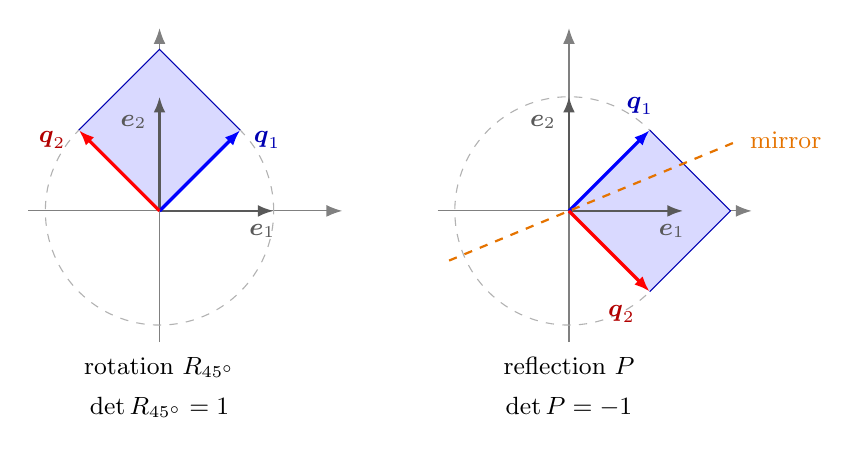
\begin{tikzpicture}[font=\small, >={Latex[length=2mm]}, x=1.45cm, y=1.45cm]
  \foreach \panel/\sx/\sy/\pname/\dval in {0/-1/1/{rotation $R_{45^\circ}$}/{$\det R_{45^\circ}=1$}, 1/1/-1/{reflection $P$}/{$\det P=-1$}} {
  \begin{scope}[xshift=\panel*5.2cm]
    % axes and unit circle
    \draw[->, gray] (-1.15,0) -- (1.6,0);
    \draw[->, gray] (0,-1.15) -- (0,1.6);
    \draw[gray!60, thin, dashed] (0,0) circle (1);
    % image of the unit square
    \fill[blue!15] (0,0) -- (0.7071,0.7071) -- ({0.7071+\sx*0.7071},{0.7071+\sy*0.7071}) -- ({\sx*0.7071},{\sy*0.7071}) -- cycle;
    \draw[blue!70!black, thin] (0.7071,0.7071) -- ({0.7071+\sx*0.7071},{0.7071+\sy*0.7071}) -- ({\sx*0.7071},{\sy*0.7071});
    % standard basis
    \draw[->, gray!70!black, thick] (0,0) -- (1,0);
    \draw[->, gray!70!black, thick] (0,0) -- (0,1);
    \node[gray!70!black, anchor=north] at (0.9,-0.03) {$\boldsymbol{e}_1$};
    \node[gray!70!black, anchor=east] at (-0.03,0.78) {$\boldsymbol{e}_2$};
    % images of e_1, e_2 = columns of the matrix
    \draw[->, blue, very thick] (0,0) -- (0.7071,0.7071);
    \draw[->, red, very thick] (0,0) -- ({\sx*0.7071},{\sy*0.7071});
    \node[below, black] at (0,-1.2) {\pname};
    \node[below, black] at (0,-1.55) {\dval};
  \end{scope}
  }
  % left panel labels
  \node[blue!70!black, anchor=west] at (0.74,0.62) {$\boldsymbol{q}_1$};
  \node[red!70!black, anchor=east] at (-0.74,0.62) {$\boldsymbol{q}_2$};
  % right panel labels and mirror line
  \begin{scope}[xshift=5.2cm]
    \draw[orange!90!black, thick, dashed] (-1.05,-0.435) -- (1.5,0.621);
    \node[orange!90!black, anchor=west] at (1.5,0.621) {mirror};
    \node[blue!70!black, anchor=south] at (0.62,0.76) {$\boldsymbol{q}_1$};
    \node[red!70!black, anchor=north east] at (0.66,-0.74) {$\boldsymbol{q}_2$};
  \end{scope}
\end{tikzpicture}
\end{document}
